\documentclass[12pt]{article}
\usepackage{url,amsmath,setspace,amssymb,amsthm,amsfonts}


\setlength{\oddsidemargin}{.25in}
\setlength{\evensidemargin}{.25in}
\setlength{\textwidth}{6.25in}
\setlength{\topmargin}{-0.4in}
\setlength{\textheight}{8.5in}

\newcommand{\heading}[5]{
   \renewcommand{\thepage}{#1-\arabic{page}}
   \noindent
   \begin{center}
   \framebox[\textwidth]{
     \begin{minipage}{0.9\textwidth} \onehalfspacing
       {\bf CS 290G -- Introduction to Modern Cryptography} \hfill #2

       {\centering \Large #5
       
       }\medskip

       {\it #3 \hfill #4}
     \end{minipage}
   }
   \end{center}
}

\newcommand{\handout}[3]{\heading{#1}{#2}{Instructor:
Stefano Tessaro}{Scribe: Shiyu Ji}{Lecture #1: #3}}

\setlength{\parindent}{0in}

\newcommand{\eqdef}{\stackrel{def}{=}}
\newcommand{\N}{\mathbb{N}}
\newcommand{\R}{\mathbb{R}}
\newcommand{\Z}{\mathbb{Z}}
\newcommand{\F}{\mathbb{F}}
\newcommand{\bits}{\{0,1\}}
\newcommand{\inr}{\in_{\mbox{\tiny R}}}
%\newcommand{\getsr}{\gets_{\mbox{\tiny R}}}
\newcommand{\getsr}{\stackrel{\$}{\gets}}
\newcommand{\st}{\mbox{ s.t. }}
\newcommand{\etal}{{\it et al }}
\newcommand{\into}{\rightarrow}

\newcommand{\Ex}{\mathbb{E}}
\newcommand{\e}{\epsilon}
\newcommand{\ee}{\varepsilon}
\newcommand{\ceil}[1]{{\lceil{#1}\rceil}}
\newcommand{\floor}[1]{{\lfloor{#1}\rfloor}}
\newcommand{\angles}[1]{\langle #1 \rangle}
\newcommand{\Com}{{\sf Com}}
\newcommand{\desc}{{\sf desc}}

\newcommand{\rightstep}[1]{%
$\underrightarrow{\quad #1 \quad}$ }

\newcommand{\leftstep}[1]{%
$\underleftarrow{\quad #1 \quad}$ }

\newcommand{\Adv}{\mathsf{Adv}}

\newcommand{\tab}{\hspace{0.3in}}
%%%%%%%%%%%%%%%%%%%%%%%%%%%%
% Theorems & Definitions


\newtheorem{theorem}{Theorem}[section]

\newtheorem{claim}[theorem]{Claim}
\newtheorem{subclaim}{Claim}[theorem]
\newtheorem{proposition}[theorem]{Proposition}
\newtheorem{lemma}[theorem]{Lemma}
\newtheorem{corollary}[theorem]{Corollary}
\newtheorem{conjecture}[theorem]{Conjecture}
\newtheorem{observation}[theorem]{Observation}

\theoremstyle{definition}
\newtheorem{definition}[theorem]{Definition}
\newtheorem{construction}[theorem]{Construction}
\newtheorem{example}[theorem]{Example}
\newtheorem{algorithm1}[theorem]{Algorithm}
\newtheorem{protocol}[theorem]{Protocol}
\newtheorem{remark}[theorem]{Remark}
\newtheorem{assumption}[theorem]{Assumption}
\newtheorem{fact}[theorem]{Fact}

%\bibliographystyle{plain}
\usepackage{tikz}
\usetikzlibrary{calc,decorations.pathreplacing}

\begin{document}
\handout{4}{Jan 19, 2016}{Hardcore Predicates}
\section{Recap}
Last lecture we defined Pseudorandom Generator (PRG). That is, PRG is a function family 
$G : \bits^\lambda \mapsto \bits^{n(\lambda)}$, where $n(\lambda) > \lambda$, such that for all PPT distinguisher $D$, the advantage
$$\Adv_{G, \lambda}^{prg} (D) \eqdef \bigg| \Pr[s \getsr \bits^\lambda : D(G(s)) = 1] - \Pr[y \getsr \bits^{n(\lambda)} : D(y) = 1] \bigg|$$
is negligible in $\lambda$.

\section{Hardcore Predicates}
To build PRG from one-way permutation (OWP), we need hardcore predicates. 
Informally, given a family of one-way functions $f : \bits^\lambda \mapsto \bits^{\lambda'}$ and a family of predicates $P : \bits^\lambda \mapsto \bits$, we say $P$ is a hardcore predicate for $f$ if given $f(x)$ for $x \getsr \bits^\lambda$, it is hard to predict $P(x)$.

We can formalize the intuition as following.
\begin{definition}
$P$ is a {\bf hardcore predicate} for OWF $f$, if for all PPT adversary $A$,
$$\Adv_{f,P,\lambda}^{pred} (A) \eqdef 2 \bigg| \Pr[x \getsr \bits^\lambda : A(f(x)) = P(x)] - \frac{1}{2} \bigg|$$
is negligible in $\lambda$.
\end{definition}
Let us see how to construct a hardcore predicate.
Assume the functions $f$ as above. We build another function family $g^f : \bits^{2\lambda} \mapsto \bits^{\lambda + \lambda'}$ defined by
$$g^f (x, r) \eqdef (f(x), r).$$
In Lecture 2, we have shown that if $f$ is OWF, then so is $g^f$.

Goldreich and Levin \cite{GL89} have given a hardcore predicate that can be constructed from any such OWF.
\begin{theorem}
If $f$ is OWF, then $P(x, r) = \angles{x, r}$ is a hardcore predicate for $g^f$, where the inner product is defined as
$$\angles{x, r} \eqdef \sum_{i=1}^\lambda x_ir_i \mod 2.$$
\end{theorem}
A little example for the inner product is: let $x=101$ and $r=111$, then $\angles{x,r} = 1\cdot 1 + 0\cdot 1 + 1\cdot 1 \mod 2 = 0$.

Blum and Micali \cite{BM84} have given a concrete construction of hardcore predicate, assuming the hardness of Discrete Logarithm Problem.
\begin{theorem}
For a multiplicative group $\Z_p^*$ with a large prime $p$ and a generator $g$, given a function $f(x) \eqdef g^x \mod p$, define the predicate for $f$ as the most significant bit (MSB) of $x$:
$$P(x) = MSB(x) \eqdef \begin{cases}
1, & \textrm{if } x>\frac{p-1}{2}, \\
0, & \textrm{if } x\leq\frac{p-1}{2}.
\end{cases}.$$
Then $P$ is a hardcore predicate, assuming $f$ is one-way (by DLP).
\end{theorem}

\section{Predicting iff Distinguishing}
Given a OWF $f$ and a predicate $P$, there are two distributions on strings with length $\lambda' + 1$:
\begin{itemize}
\item $P_0$: $x \getsr \bits^\lambda$, return $(f(x), P(x))$.
\item $P_1$: $x \getsr \bits^\lambda$, $u \getsr \bits$, return $(f(x), u)$.
\end{itemize}
If $P$ is a hardcore predicate, can any efficient adversary distinguish these two distributions? The answer is no.
\begin{lemma}
\label{lem:pred}
If $P$ is a hardcore predicate for $f$, then the advantage $\Adv_{P_0,P_1,\lambda}^{dist}(D)$ is negligible for all PPT $D$.
\end{lemma}

Now we consider the case $f : \bits^\lambda \mapsto \bits^{\lambda'}$ is one-way permutation, i.e., $\lambda = \lambda'$ and $f$ is one-to-one.
The following theorem constructs a PRG given a OWP and its hardcore predicate.
\begin{theorem}
Given a function $f$ and a hardcore predicate $P$ for $f$, define $G^f : \bits^\lambda \mapsto \bits^{\lambda+1}$ as
$$G^f(x) \eqdef (f(x), P(x)).$$
If $f$ is OWP, then $G^f$ is a PRG.
\end{theorem}
\begin{proof}
Let $D$ be any distinguisher.
$$\begin{aligned}
&\Adv_{G^f, \lambda}^{prg}(D) 
=\bigg| \Pr[s \getsr \bits^\lambda : D(G^f(s)) = 1] - \Pr[y \getsr \bits^{\lambda+1} : D(y) = 1] \bigg| \\
=&\bigg| \Pr[s \getsr \bits^\lambda : D(f(s), P(s)) = 1] - \Pr[s \getsr \bits^\lambda, u \getsr \bits : D(f(s), u) = 1] \\
&+ \Pr[s \getsr \bits^\lambda, u \getsr \bits : D(f(s), u) = 1] - \Pr[y \getsr \bits^{\lambda+1} : D(y) = 1] \bigg|.
\end{aligned}$$
Define
$$\Delta_1 \eqdef \Pr[s \getsr \bits^\lambda : D(f(s), P(s)) = 1] - \Pr[s \getsr \bits^\lambda, u \getsr \bits : D(f(s), u) = 1],$$
$$\Delta_2 \eqdef \Pr[s \getsr \bits^\lambda, u \getsr \bits : D(f(s), u) = 1] - \Pr[y \getsr \bits^{\lambda+1} : D(y) = 1].$$
Hence 
$$\Adv_{G^f, \lambda}^{prg}(D) = |\Delta_1 + \Delta_2| \leq |\Delta_1| + |\Delta_2|.$$
Note that since $P(s)$ is a hardcore predicate, by Lemma \ref{lem:pred} it follows that $|\Delta_1|$ is negligible. Since $f$ is OWP, if $s$ is uniformly distributed over $\bits^\lambda$, then so is $f(s)$. Thus $\Delta_2 = 0$. It follows that $\Adv_{G^f, \lambda}^{prg}(D)$ must be negligible for any $D$.
\end{proof}
The theorem above requires $F$ to be OWP. In fact, we can transform every OWF into a PRG \cite{HILL99}.\footnote{In \cite{HILL99} the construction is not very efficient in practical sense, making around $\lambda^3$ calls to $f$.}

\section{Extending PRG and Hybrid Argument}

\begin{figure}[!t]
\centering{}
\begin{tikzpicture}
% s_i
\draw (0,0) rectangle (1,2); \node at (0.5, 1) {$s_0$};
\draw (2,0) rectangle (3,2); \node at (2.5, 1) {$s_1$};
\draw (4,0) rectangle (5,2); \node at (4.5, 1) {$s_2$};
\draw (6,0) rectangle (7,2); \node at (6.5, 1) {$s_3$};
\draw (10,0) rectangle (11,2); \node at (10.5, 1) {$s_{t-1}$};
\draw (12,0) [fill=lightgray] rectangle (13,2); \node at (12.5, 1) {$s_t$};
% z_i
\draw [fill = lightgray] (2,2) rectangle (3,3); \node at (2.5, 2.5) {$z_1$}; 
\draw [fill = lightgray] (4,2) rectangle (5,3); \node at (4.5, 2.5) {$z_2$};
\draw [fill = lightgray] (6,2) rectangle (7,3); \node at (6.5, 2.5) {$z_3$};
\draw [fill = lightgray] (10,2) rectangle (11,3); \node at (10.5, 2.5) {$z_{t-1}$};
\draw [fill = lightgray] (12,2) rectangle (13,3); \node at (12.5, 2.5) {$z_t$};
% arrows
\draw [->, thick] (1,1) -- (2,1); \node [above] at (1.5,1) {$G$};
\draw [->, thick] (3,1) -- (4,1); \node [above] at (3.5,1) {$G$};
\draw [->, thick] (5,1) -- (6,1); \node [above] at (5.5,1) {$G$};
\draw [->, thick] (7,1) -- (8,1); \node [above] at (7.5,1) {$G$};
\node at (8.5,1) {$\cdots$};
\draw [->, thick] (9,1) -- (10,1); \node [above] at (9.5,1) {$G$};
\draw [->, thick] (11,1) -- (12,1); \node [above] at (11.5,1) {$G$};
% misc
\draw [decorate,decoration={brace, amplitude=7pt}] (0,0) -- (0,2);
\node [left] at (-0.2,1) {$\lambda$};
\draw [decorate,decoration={brace, amplitude=7pt}] (2,2) -- (2,3);
\node [left] at (1.8,2.5) {$k$};
\end{tikzpicture}
\caption{Extended PRG $G_t : \bits^\lambda \mapsto \bits^{\lambda+tk}$ based on $G : \bits^\lambda \mapsto \bits^{\lambda+k}$.}
\label{fig:extended_prg}
\end{figure}

Given a PRG $G : \bits^\lambda \mapsto \bits^{\lambda+k}$, $k\geq 1$, our goal is to build a PRG $G' : \bits^\lambda \mapsto \bits^{\lambda+k'}$, where $k'$ is much larger than $k$.

Given a parameter $t$ in $\N^+$, we give a construction $G_t : \bits^\lambda \mapsto \bits^{\lambda+tk}$ as following:
\begin{quote}
Algorithm $G_t (s)$, $s\in\bits^\lambda$
\begin{enumerate}
\item $s_0 \gets s$.
\item {\bf for} $i=1$ to $t$ {\bf do}
\item \tab $s_i || z_i \gets G(s_{i-1})$.
\item {\bf return} $(z_1, z_2, \cdots, z_t, s_t)$.
\end{enumerate}
\end{quote}
Figure \ref{fig:extended_prg} depicts the construction above.

We are going to argue that $G_t$ is also a PRG. The proof idea is via {\bf hybrid argument}, which will be often used!

\begin{theorem}
If $G$ is a PRG, and $t$ is polynomial in $\lambda$, then so is $G_t$.
\end{theorem}
\begin{proof}
It suffices to show that for all PPT $D$, there exists a distinguisher $D^*$ s.t.
$$\Adv_{G_t,\lambda}^{prg}(D) = t\cdot \Adv_{G,\lambda}^{prg}(D^*).$$
This is because the advantage of $D^*$ is negligible since $G$ is PRG, and $t$ is polynomial in $\lambda$. It immediately follows that $t\cdot \Adv_{G,\lambda}^{prg}(D^*)$ is also negligible.

To give the construction of $D^*$, we first define $t+1$ \emph{hybrid} distributions $H_0, H_1, \cdots, H_t$:
\begin{quote}
$H_i$: (for $i \in \{1, 2, \cdots, t\}$)
\begin{enumerate}
\item {\bf for} $j=1$ to $i$ {\bf do}
\item \tab $z_j \getsr \bits^k$.
\item $s_i \getsr \bits^\lambda$.
\item {\bf for} $j=i+1$ to $t$ {\bf do}
\item \tab $s_j||z_j \gets G(s_{j-1})$.
\item {\bf return} $(z_1, z_2, \cdots, z_t, s_t)$.
\end{enumerate}
\end{quote}
Figure \ref{fig:2h} depicts the distributions $H_i$ and $H_{i+1}$.

\begin{figure}[!t]
\centering{}
\begin{tikzpicture}
% s_i
\node at (1.3,1) {$\cdots$};
\draw (4,0) rectangle (5,2); \node at (4.5, 1) {$s_i$};
\draw (6,0) rectangle (7,2); \node at (6.5, 1) {$s_{i+1}$};
\draw (10,0) rectangle (11,2); \node at (10.5, 1) {$s_{t-1}$};
\draw (12,0) [fill = lightgray] rectangle (13,2); \node at (12.5, 1) {$s_t$};
% z_i
\draw [fill = lightgray] (-2,2) rectangle (-1,3); \node at (-1.5, 2.5) {$z_1$}; 
\draw [fill = lightgray] (-0.5,2) rectangle (0.5,3); \node at (0, 2.5) {$z_2$};
\draw [fill = lightgray] (2,2) rectangle (3,3); \node at (2.5, 2.5) {$z_{i-1}$};
\draw [fill = lightgray] (4,2) rectangle (5,3); \node at (4.5, 2.5) {$z_i$};
\draw [fill = lightgray] (6,2) rectangle (7,3); \node at (6.5, 2.5) {$z_{i+1}$};
\draw [fill = lightgray] (10,2) rectangle (11,3); \node at (10.5, 2.5) {$z_{t-1}$};
\draw [fill = lightgray] (12,2) rectangle (13,3); \node at (12.5, 2.5) {$z_t$};
% arrows
\draw [->, thick] (5,1) -- (6,1); \node [above] at (5.5,1) {$G$};
\draw [->, thick] (7,1) -- (8,1); \node [above] at (7.5,1) {$G$};
\node at (8.5,1) {$\cdots$};
\draw [->, thick] (9,1) -- (10,1); \node [above] at (9.5,1) {$G$};
\draw [->, thick] (11,1) -- (12,1); \node [above] at (11.5,1) {$G$};
% misc
\draw [decorate,decoration={brace, amplitude=7pt}] (4,0) -- (4,2);
\node [left] at (3.8,1) {$\lambda$};
\draw [decorate,decoration={brace, amplitude=7pt}] (0.5,3) -- (0.5,2);
\node [right] at (0.7,2.5) {$k$};
\node at (-1,1) {$H_i$};
\end{tikzpicture}

\hspace{.5in}

\begin{tikzpicture}
% s_i
\node at (1.3,1) {$\cdots$};
\draw (6,0) rectangle (7,2); \node at (6.5, 1) {$s_{i+1}$};
\draw (10,0) rectangle (11,2); \node at (10.5, 1) {$s_{t-1}$};
\draw (12,0) [fill = lightgray] rectangle (13,2); \node at (12.5, 1) {$s_t$};
% z_i
\draw [fill = lightgray] (-2,2) rectangle (-1,3); \node at (-1.5, 2.5) {$z_1$}; 
\draw [fill = lightgray] (-0.5,2) rectangle (0.5,3); \node at (0, 2.5) {$z_2$};
\draw [fill = lightgray] (2,2) rectangle (3,3); \node at (2.5, 2.5) {$z_{i-1}$};
\draw [fill = lightgray] (4,2) rectangle (5,3); \node at (4.5, 2.5) {$z_i$};
\draw [fill = lightgray] (6,2) rectangle (7,3); \node at (6.5, 2.5) {$z_{i+1}$};
\draw [fill = lightgray] (10,2) rectangle (11,3); \node at (10.5, 2.5) {$z_{t-1}$};
\draw [fill = lightgray] (12,2) rectangle (13,3); \node at (12.5, 2.5) {$z_t$};
% arrows
\draw [->, thick] (7,1) -- (8,1); \node [above] at (7.5,1) {$G$};
\node at (8.5,1) {$\cdots$};
\draw [->, thick] (9,1) -- (10,1); \node [above] at (9.5,1) {$G$};
\draw [->, thick] (11,1) -- (12,1); \node [above] at (11.5,1) {$G$};
% misc
\draw [decorate,decoration={brace, amplitude=7pt}] (6,0) -- (6,2);
\node [left] at (5.8,1) {$\lambda$};
\draw [decorate,decoration={brace, amplitude=7pt}] (0.5,3) -- (0.5,2);
\node [right] at (0.7,2.5) {$k$};
\node at (-1,1) {$H_{i+1}$};
\end{tikzpicture}
\caption{The distributions $H_i$ and $H_{i+1}$.}
\label{fig:2h}
\end{figure}

Note that $H_0$ is the distribution of $G_t(s)$ given $s \getsr \bits^\lambda$. $H_t$ is the uniform distribution $U_{\lambda+tk}$.

Now let us look at $H_i$ and $H_{i+1}$, $i \in \{1, 2, \cdots, t-1\}$. The only difference between $H_i$ and $H_{i+1}$ is $z_{i+1}$:
\begin{itemize}
\item $z_{i+1}$ is computed through $G$ in $H_i$.
\item $z_{i+1}$ is uniformly random in $H_{i+1}$.
\end{itemize}
Thus if $G$ is PRG, then $H_i$ and $H_{i+1}$ are computationally indistinguishable.

Based on the motivation above, we build $D^*$ as following:
\begin{quote}
Distinguisher $D^* (y)$: ($y \in \bits^{\lambda+k}$, $G : \bits^\lambda \mapsto \bits^{\lambda+k}$)
\begin{enumerate}
\item $i \getsr \{1, 2, \cdots, t\}$.
\item {\bf for} $j=1$ to $i-1$ {\bf do}
\item \tab $z_j \getsr \bits^k$.
\item $(s_i, z_i) \gets y$.
\item {\bf for} $j=i+1$ to $t$ {\bf do}
\item \tab $(s_j, z_j) \gets G(s_{j-1})$.
\item $b \getsr D(z_1, z_2, \cdots, z_t, s_t)$.
\item {\bf output} $b$.
\end{enumerate}
\end{quote}
Let $D_i^*$ be $D^*$ with fixed $i$. Then the advantage of $D^*$ is
$$\begin{aligned}
&\Adv_{G,\lambda}^{prg}(D^*) \\
=& \bigg| \Pr[s \getsr \bits^\lambda : D^*(G(s)) = 1] - \Pr[y \getsr \bits^{\lambda+k} : D^*(y) = 1] \bigg| \\
=& \bigg| \frac{1}{t}\sum_{i=1}^t \Pr[s \getsr \bits^\lambda : D_i^*(G(s)) = 1] - \frac{1}{t}\sum_{i=1}^t \Pr[y \getsr \bits^{\lambda+k} : D_i^*(y) = 1] \bigg| \\
=& \frac{1}{t}\bigg| \sum_{i=1}^t \Pr[s \getsr \bits^\lambda : D_i^*(G(s)) = 1] - \sum_{i=1}^t \Pr[y \getsr \bits^{\lambda+k} : D_i^*(y) = 1] \bigg| \\
\end{aligned}$$
Define
$$p_i \eqdef \Pr[s \getsr \bits^\lambda : D_i^*(G(s)) = 1].$$
$$q_i \eqdef \Pr[y \getsr \bits^{\lambda+k} : D_i^*(y) = 1].$$
We claim that
\begin{enumerate}
\item $p_i = \Pr[D(H_{i-1}) = 1]$.
\item $q_i = \Pr[D(H_i) = 1]$.
\end{enumerate}
Then it follows that $q_i = p_{i+1}$. Thus
$$\Adv_{G,\lambda}^{prg}(D^*) = \frac{1}{t}|p_1 - q_t| = \frac{1}{t} \Adv_{G_t, \lambda}^{prg}(D).$$
\end{proof}
The proof of the claims above will be given next lecture.

\begin{thebibliography}{10}
\bibitem{HILL99} 
J. H\aa stad, R. Impagliazzo, L.A. Levin and M. Luby, 1999. 
A pseudorandom generator from any one-way function. 
SIAM Journal on Computing, 28(4), pp. 1364-1396.
	
\bibitem{GL89}
O. Goldreich and L.A. Levin, 1989, February. 
A hard-core predicate for all one-way functions. 
In Proceedings of the twenty-first annual ACM symposium on Theory of computing (pp. 25-32). ACM.

\bibitem{BM84}
M. Blum and S. Micali, 1984. 
How to generate cryptographically strong sequences of pseudorandom bits. 
SIAM journal on Computing, 13(4), pp. 850-864.
\end{thebibliography}

\end{document}
